%%%%%%%%%%%%%%%%%%%%%%%%%%%%%%%%%%%%%%%%%
% Short Sectioned Assignment LaTeX Template Version 1.0 (5/5/12)
% This template has been downloaded from: http://www.LaTeXTemplates.com
% Original author:  Frits Wenneker (http://www.howtotex.com)
% License: CC BY-NC-SA 3.0 (http://creativecommons.org/licenses/by-nc-sa/3.0/)
%%%%%%%%%%%%%%%%%%%%%%%%%%%%%%%%%%%%%%%%%

%----------------------------------------------------------------------------------------
%	PACKAGES AND OTHER DOCUMENT CONFIGURATIONS
%----------------------------------------------------------------------------------------

\documentclass[paper=a4, fontsize=11pt]{scrartcl} % A4 paper and 11pt font size

% ---- Entrada y salida de texto -----

\usepackage{array}
\usepackage{booktabs}
\usepackage{tabulary}
\usepackage{multirow}

\usepackage{color}
\usepackage{listings}
\usepackage[T1]{fontenc} % Use 8-bit encoding that has 256 glyphs
\usepackage[utf8]{inputenc}
%\usepackage{fourier} % Use the Adobe Utopia font for the document - comment this line to return to the LaTeX default
\usepackage{footnote}
\usepackage{eurosym}
\usepackage{eurosym} % Sirve para poner \euro y que salga el símbolo del €.

% ---- Idioma --------
 
\usepackage[spanish, es-tabla]{babel} % Selecciona el español para palabras introducidas automáticamente, p.ej. "septiembre" en la fecha y especifica que se use la palabra Tabla en vez de Cuadro

% ---- Otros paquetes ----
\usepackage{subfig}
\usepackage{url} % ,href} %para incluir URLs e hipervínculos dentro del texto (aunque hay que instalar href)
\usepackage{amsmath,amsfonts,amsthm} % Math packages
%\usepackage{graphics,graphicx, floatrow} %para incluir imágenes y notas en las imágenes
\usepackage{graphics,graphicx, float} %para incluir imágenes y colocarlas

% Para hacer tablas comlejas
%\usepackage{multirow}
%\usepackage{threeparttable}

%\usepackage{sectsty} % Allows customizing section commands
%\allsectionsfont{\centering \normalfont\scshape} % Make all sections centered, the default font and small caps

\usepackage{fancyhdr} % Custom headers and footers
\pagestyle{fancyplain} % Makes all pages in the document conform to the custom headers and footers
\fancyhead{} % No page header - if you want one, create it in the same way as the footers below
\fancyfoot[L]{} % Empty left footer
\fancyfoot[C]{} % Empty center footer
\fancyfoot[R]{\thepage} % Page numbering for right footer
\renewcommand{\headrulewidth}{0pt} % Remove header underlines
\renewcommand{\footrulewidth}{0pt} % Remove footer underlines
\setlength{\headheight}{13.6pt} % Customize the height of the header

\numberwithin{equation}{section} % Number equations within sections (i.e. 1.1, 1.2, 2.1, 2.2 instead of 1, 2, 3, 4)
\numberwithin{figure}{section} % Number figures within sections (i.e. 1.1, 1.2, 2.1, 2.2 instead of 1, 2, 3, 4)
\numberwithin{table}{section} % Number tables within sections (i.e. 1.1, 1.2, 2.1, 2.2 instead of 1, 2, 3, 4)

\setlength\parindent{0pt} % Removes all indentation from paragraphs - comment this line for an assignment with lots of text

\newcommand{\horrule}[1]{\rule{\linewidth}{#1}} % Create horizontal rule command with 1 argument of height


\title{	
	\normalfont \normalsize 
	\textsc{\textbf{Inteligencia de Negocio (2017-2018)} \\ Grado en Ingeniería Informática \\ Universidad de Granada} \\ [25pt] 
	\horrule{0.5pt} \\[0.4cm]
	\huge Práctica 2 \\
	\horrule{2pt} \\[0.5cm]
}

\author{Juan José Sierra González \\ jjsierra103@gmail.com}

\date{\normalsize\today}

\begin{document}
	\maketitle
	\thispagestyle{empty}
	
	\newpage
	
	\tableofcontents
	
	\listoffigures
	
	\listoftables
	
	\newpage
	
	\section{Introducción}
	En esta práctica se tratará de interpretar el comportamiento de distintos algoritmos de clustering, trabajando sobre una base de datos de accidentes en España en el año 2013. Eligiendo distintos subconjuntos del conjunto total de datos se elaborarán 3 casos de estudio sobre los que ejecutar los algoritmos. Estos algoritmos de clustering seleccionados para el estudio son \textbf{K-Means, DBSCAN, Spectral Clustering, Birch y Ward}.\\
	
	Para cada caso de estudio se mostrarán las tablas de resultados y algunas gráficas ilustrativas y se tratará de dar la visión e interpretación más adecuada de las mismas.
	
	\section{Caso de estudio 1}
	
	\subsection{¿Qué se analiza?}
	En el primero de estos casos de estudio se van a analizar los \textbf{accidentes que han tenido lugar en autovías y autopistas}. Las características seleccionadas para el estudio han sido el número de vehículos implicados, el número de heridos graves y leves, el número de fallecidos y el total de víctimas afectadas. Se comprobará cuántos vehículos suelen verse involucrados en estos accidentes y cómo se distribuyen las cifras de heridos y víctimas mortales, es decir, tratar de valorar si la cifra de fallecidos en accidentes de este ámbito representa un dato sustancial frente al total de accidentes o son una pequeña muestra dentro de los accidentes registrados.\\
	
	Este caso de estudio en cuestión cuenta con 11943 ejemplos. Es el más vasto de los que se van a estudiar,
	
	\subsection{Resultados de los algoritmos}
	En este correspondiente apartado para cada caso de estudio se mostrará una tabla que recoja algunos resultados analíticos del comportamiento de los distintos algoritmos de clustering sobre el subconjunto de datos que representa el caso de estudio. En la tabla se incluyen el número de clusters en los que el algoritmo ha segmentado los ejemplos, el tiempo de ejecución y los scores obtenidos según las métricas de Calinski-Harabaz y Silhouette (estos no son calculados para el algoritmo de clustering jerárquico del estudio, el Ward). Además, para cada caso de estudio se han realizado unos filtros a los clusters, para que aquellos que tienen menos de un determinado número pequeño de ejemplos no se consideren representativos y no formen parte de los cómputos de las matrices de dispersión y los mapas de calor. En la tabla se incluyen el número de clusters que ha quedado después del filtrado y el número de ejemplos que se encontraban dentro de los clusters eliminados.\\
	
	Puesto que contaremos con un número de ejemplos muy variado entre casos de estudio, el criterio que he seguido para el filtrado de los clusters ha sido el siguiente:
	\begin{itemize}
		\item Si el conjunto de datos tiene más de 100 ejemplos, eliminar aquellos clusters que no representen el 1\% de la población.
		\item Si el conjunto de datos no supera los 100 ejemplos, eliminar aquellos clusters que representan 2 ejemplos o menos.
	\end{itemize}

	A continuación se muestra la tabla de resultados del primer caso de estudio.
	
	\begin{table}[H]
		\centering
		\resizebox{\textwidth}{!}{
			$\begin{tabular}{ *{7}{c} }
			\toprule
			\textbf{Algorithm} & \textbf{Clusters} & \textbf{Execution time} & \textbf{CH Score} & \textbf{Silhouette Score} & \textbf{Clusters after filtering} & \textbf{Number of samples dropped}\\
			\midrule
			K-Means & 4 & 0.349 & 17443.397 & 0.74487 & 4 & 0 \\			
			DBSCAN & 26 & 0.895 & 322.707 & 0.31788 & 3 & 530 \\			
			Birch & 4 & 0.374 & 10526.549 & 0.67967 & 3 & 91 \\			
			Spectral Clustering & 4 & 53.784 & 13864.674 & 0.71842 & 4 & 0 \\			
			Ward & 100 & 3.251 & - & - & 10 & 1186 \\
			\bottomrule
			\end{tabular}$
		}
		\caption{Resultados de los algoritmos de clustering para el primer caso de estudio.}
		\label{tablaTodos1}
	\end{table}

	En primer lugar será necesario explicar qué representan las métricas Calinski-Harabaz y Silhouette, para poder realizar un análisis suficientemente explicativo.\\
	
	La métrica \textbf{Calinski-Harabaz} valora para cada algoritmo la similitud entre los ejemplos dentro de un mismo cluster y la diferenciación con el resto de clusters. Dicho de otra forma, refleja un valor real que es mejor cuanta mayor similitud haya intra-cluster y menor haya entre-cluster. A mayor valor Calinski-Harabaz, mejor separados están los ejemplos de la población para k-clusters.\\
	
	La métrica \textbf{Silhouette} valora en cierto modo la misma situación que el Calinski-Harabaz, pero tratando especialmente la distancia que hay entre el ejemplo más lejano del mismo cluster y el ejemplo más cercano de un cluster diferente. En este caso se obtendrá una valoración Silhouette que siempre estará en el intervalo [-1,1], y que a mayor valor indica una mejor distribución de los ejemplos entre los clusters.\\

	El algoritmo \textbf{Ward} no tendrá valoración en las métricas debido a problemas surgidos en tiempo de ejecución, por lo que su estudio será puramente analítico basándose en el resto del contenido de las tablas y las representaciones gráficas en las que merezca la pena apoyarse.

	Para cada caso de estudio se centrará el análisis sobre un par de algoritmos, para no extender demasiado el contenido de la memoria. Para estos algoritmos se mostrarán una matriz de dispersión y un mapa de calor (\textit{heatmap}).\\

	De acuerdo a lo explicado y viendo los resultados de la tabla anterior, parece que los algoritmos que mejor separan los ejemplos en clusters son el K-Means y el Spectral Clustering, y además se observa que existe una relación casi proporcional entre las dos métricas. Sin embargo como K-Means y Spectral Clustering representan los ejemplos en el mismo número de clusters y sin filtrar nada, no veo tan interesante analizar ambos, y voy a analizar \textbf{K-Means} y \textbf{Birch}, que realizando un filtrado de un cluster obtiene una valoración relativamente buena, y que es un algoritmo que tradicionalmente trabaja bien con grandes cantidades de datos, así que lo voy a aplicar sobre el mayor subconjunto.

	\subsubsection{K-Means}
	En primer lugar se incluye la matriz de dispersión del algortimo K-Means.
	
	\begin{figure}[H]
		\centering
		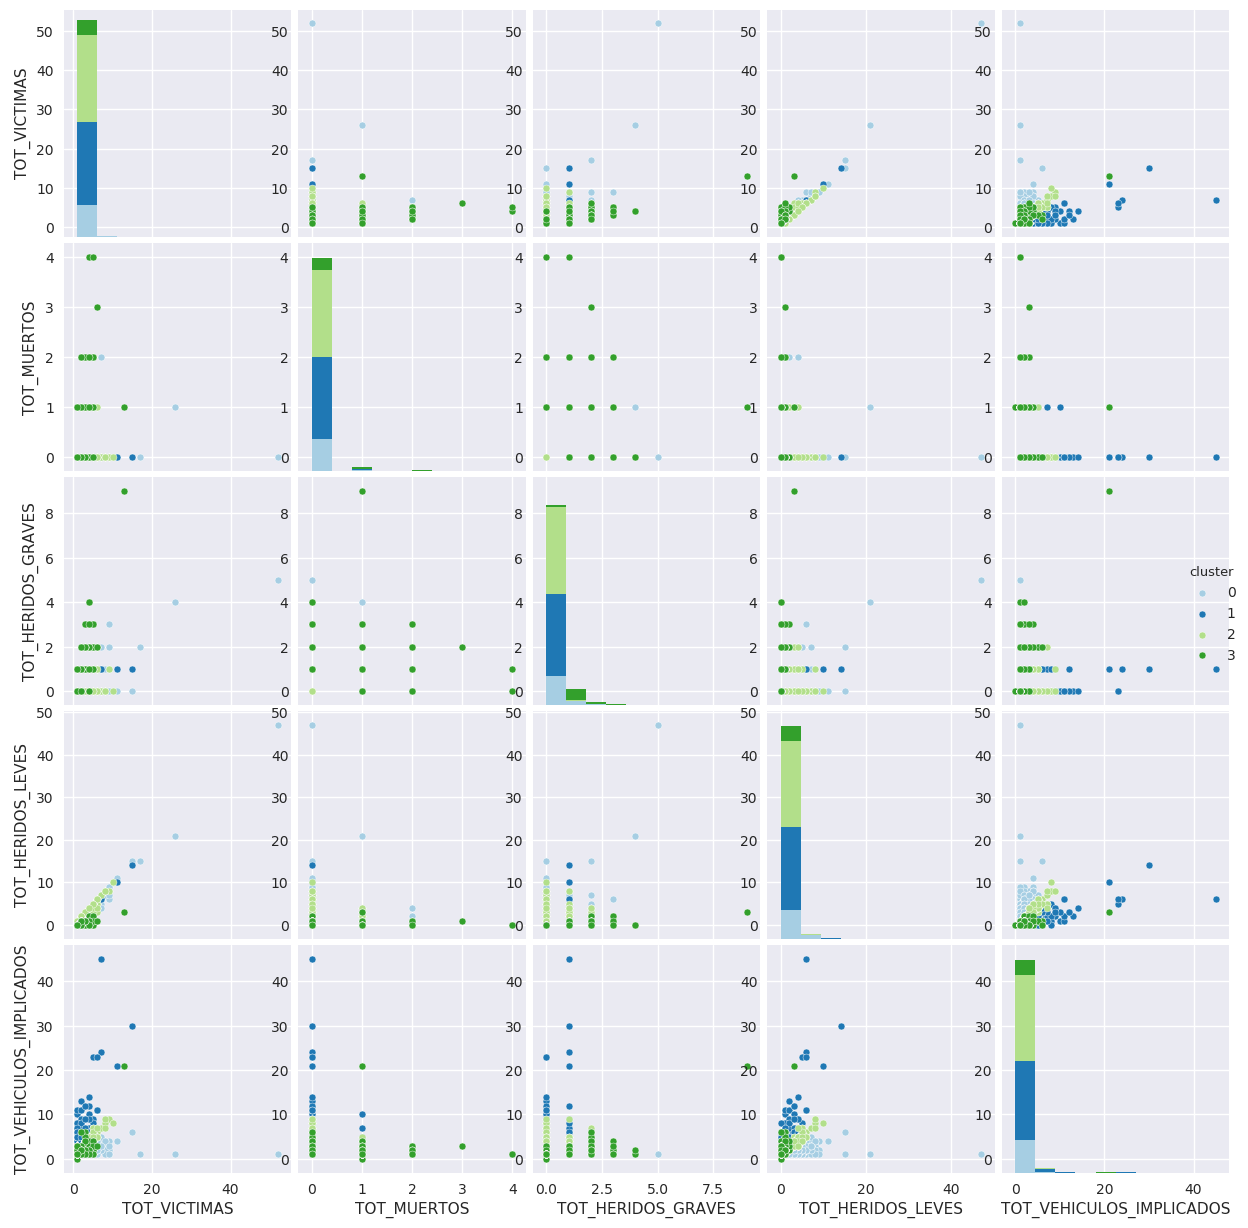
\includegraphics[scale=0.5]{plots/K-Means-HighwayAccidents-ScatterMatrix.png}
		\caption{Matriz de dispersión del algoritmo K-Means para el primer caso de estudio.}
	\end{figure}

	Para ayudar a la interpretación de la matriz de dispersión se ha incluido una tabla que comprende los valores medios de cada variable a estudiar para cada uno de los clusters que han quedado tras el filtrado, que son los mismos que se muestran en la gráfica anterior.

	\begin{table}[H]
		\centering
		\resizebox{\textwidth}{!}{
			\begin{tabular}{*{6}{c}}
				\toprule
				\textbf{CLUSTER} &  \textbf{TOT\_HERIDOS\_GRAVES} &  \textbf{TOT\_HERIDOS\_LEVES} &  \textbf{TOT\_MUERTOS} &  \textbf{TOT\_VEHICULOS\_IMPLICADOS} &  \textbf{TOT\_VICTIMAS} \\
				\midrule
				\textbf{0} &            0.140774 &           2.958497 &     0.018508 &                  1.453730 &      3.117779 \\
				\textbf{1} &            0.009233 &           1.143548 &     0.013410 &                  2.563860 &      1.166190 \\
				\textbf{2} &            0.005417 &           1.444375 &     0.003333 &                  1.451667 &      1.453125 \\
				\textbf{3} &            1.039457 &           0.146732 &     0.209618 &                  1.579531 &      1.395808 \\
				\bottomrule
			\end{tabular}
		}
		\caption{Tabla de valores medios del algoritmo K-Means para el primer caso de estudio.}
	\end{table}
	
	Por último, también se incluye un heatmap para mostrar cómo se distribuyen los valores de cada variable entre los clusters de una forma más ilustrativa. En este caso se representan los clusters contra las variables, y en cada casilla aparece el valor medio normalizado para dicha variable.
	
	\begin{figure}[H]
		\centering
		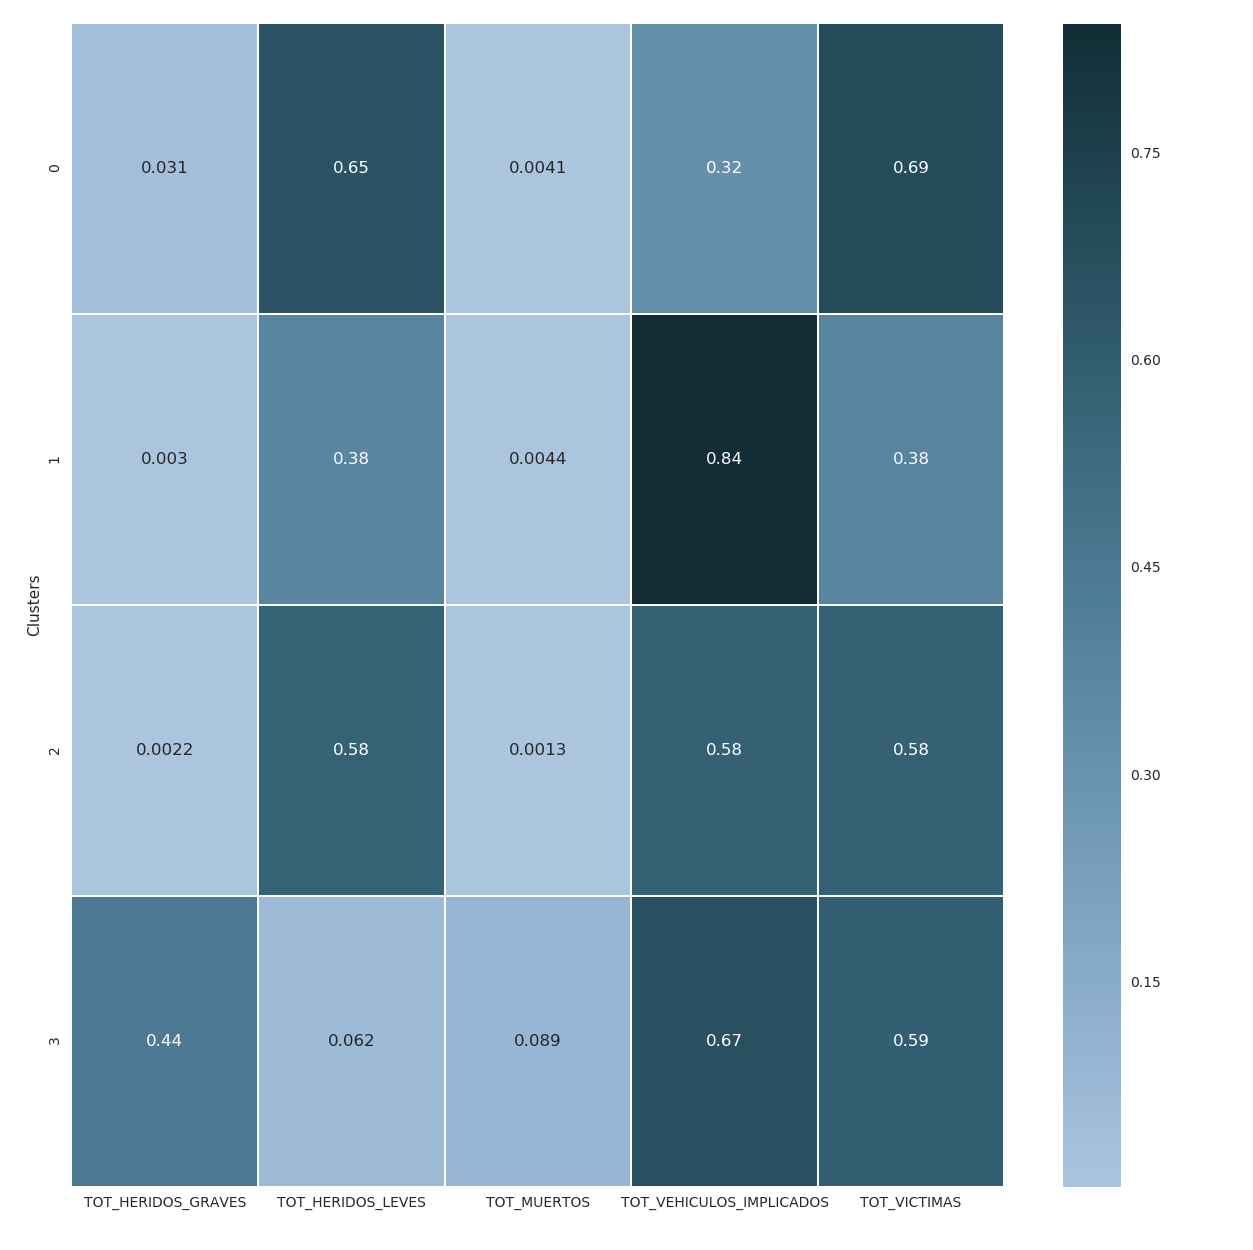
\includegraphics[scale=0.4]{heatmaps/K-Means-HighwayAccidents-Heatmap.png}
		\caption{Heatmap del algoritmo K-Means para el primer caso de estudio.}
	\end{figure}

	\subsubsection{Birch}
	A continuación se incluye la matriz de dispersión del algoritmo Birch para este primer caso de estudio.
	
	\begin{figure}[H]
		\centering
		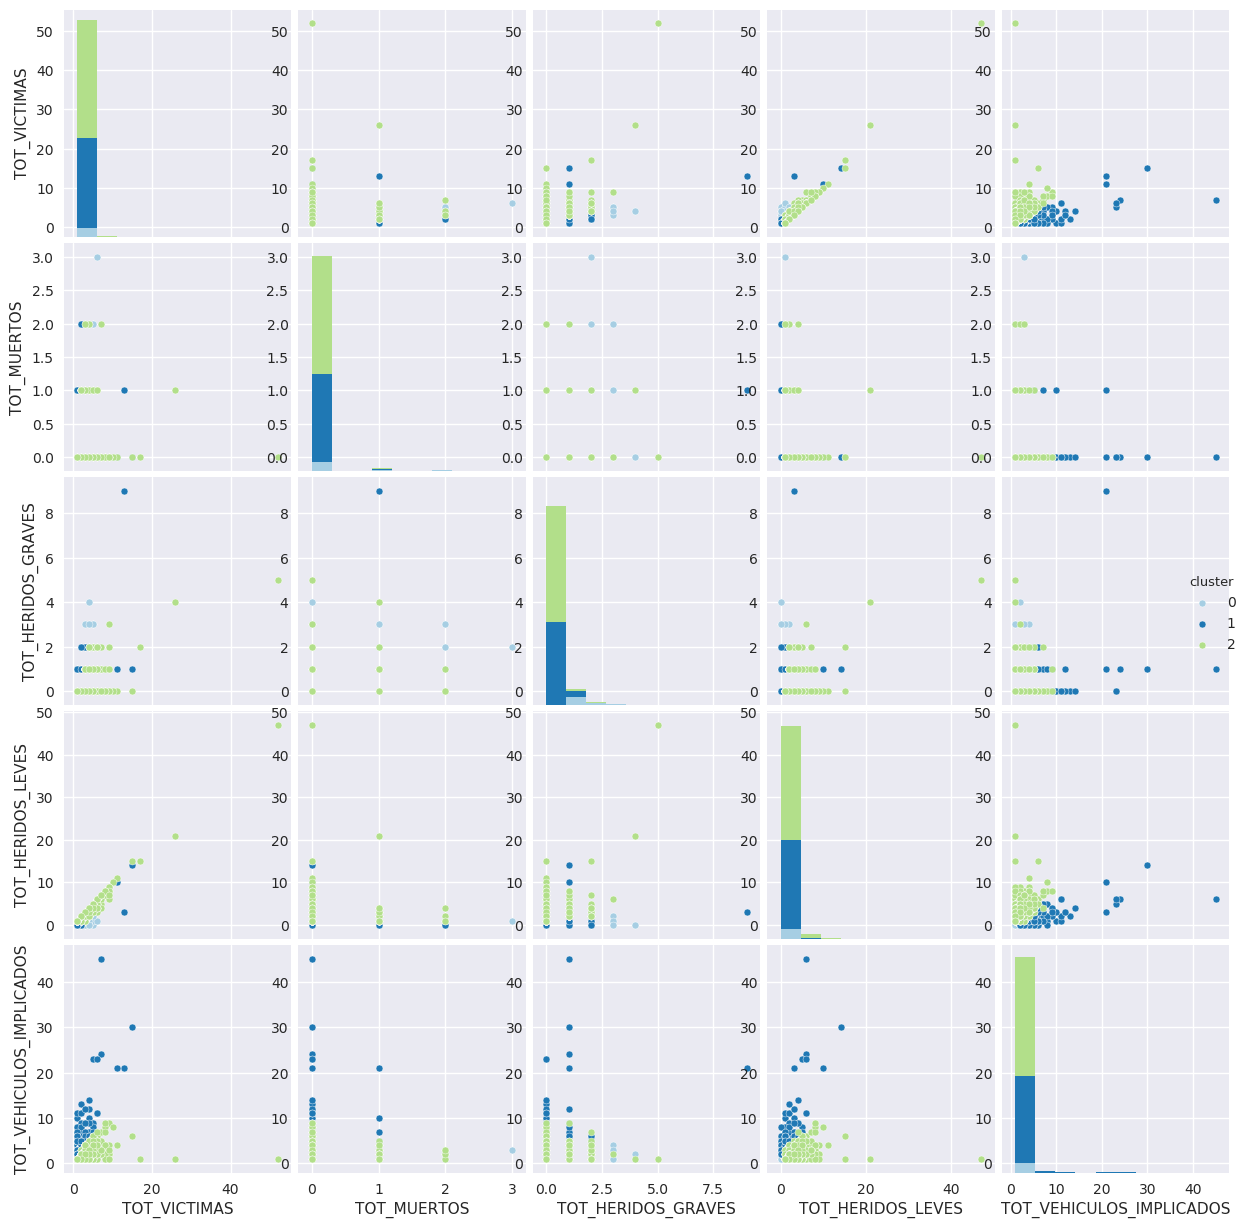
\includegraphics[scale=0.5]{plots/Birch-HighwayAccidents-ScatterMatrix.png}
		\caption{Matriz de dispersión del algoritmo Birch para el primer caso de estudio.}
	\end{figure}

	Ahora se muestra la tabla de valores medios por variable para cada cluster dentro de este caso de estudio.
	
	\begin{table}[H]
		\centering
		\resizebox{\textwidth}{!}{
			\begin{tabular}{*{6}{c}}
				\toprule
				\textbf{CLUSTER} &  \textbf{TOT\_HERIDOS\_GRAVES} &  \textbf{TOT\_HERIDOS\_LEVES} &  \textbf{TOT\_MUERTOS} &  \textbf{TOT\_VEHICULOS\_IMPLICADOS} &  \textbf{TOT\_VICTIMAS} \\
				\midrule
				\textbf{0} &            1.216433 &           0.278557 &     0.124248 &                  1.166333 &      1.619238 \\
				\textbf{1} &            0.077951 &           1.089264 &     0.012341 &                  2.545455 &      1.179556 \\
				\textbf{2} &            0.026960 &           1.863195 &     0.007857 &                  1.456632 &      1.898013 \\
				\bottomrule
			\end{tabular}
		}
		\caption{Tabla de valores medios del algoritmo Birch para el primer caso de estudio.}
	\end{table}

	Y por último, también se muestra el heatmap que representa el valor medio normalizado por cada variable para cada uno de los clusters, para ayudar a visualizar la tabla anterior de forma más clara.

	\begin{figure}[H]
		\centering
		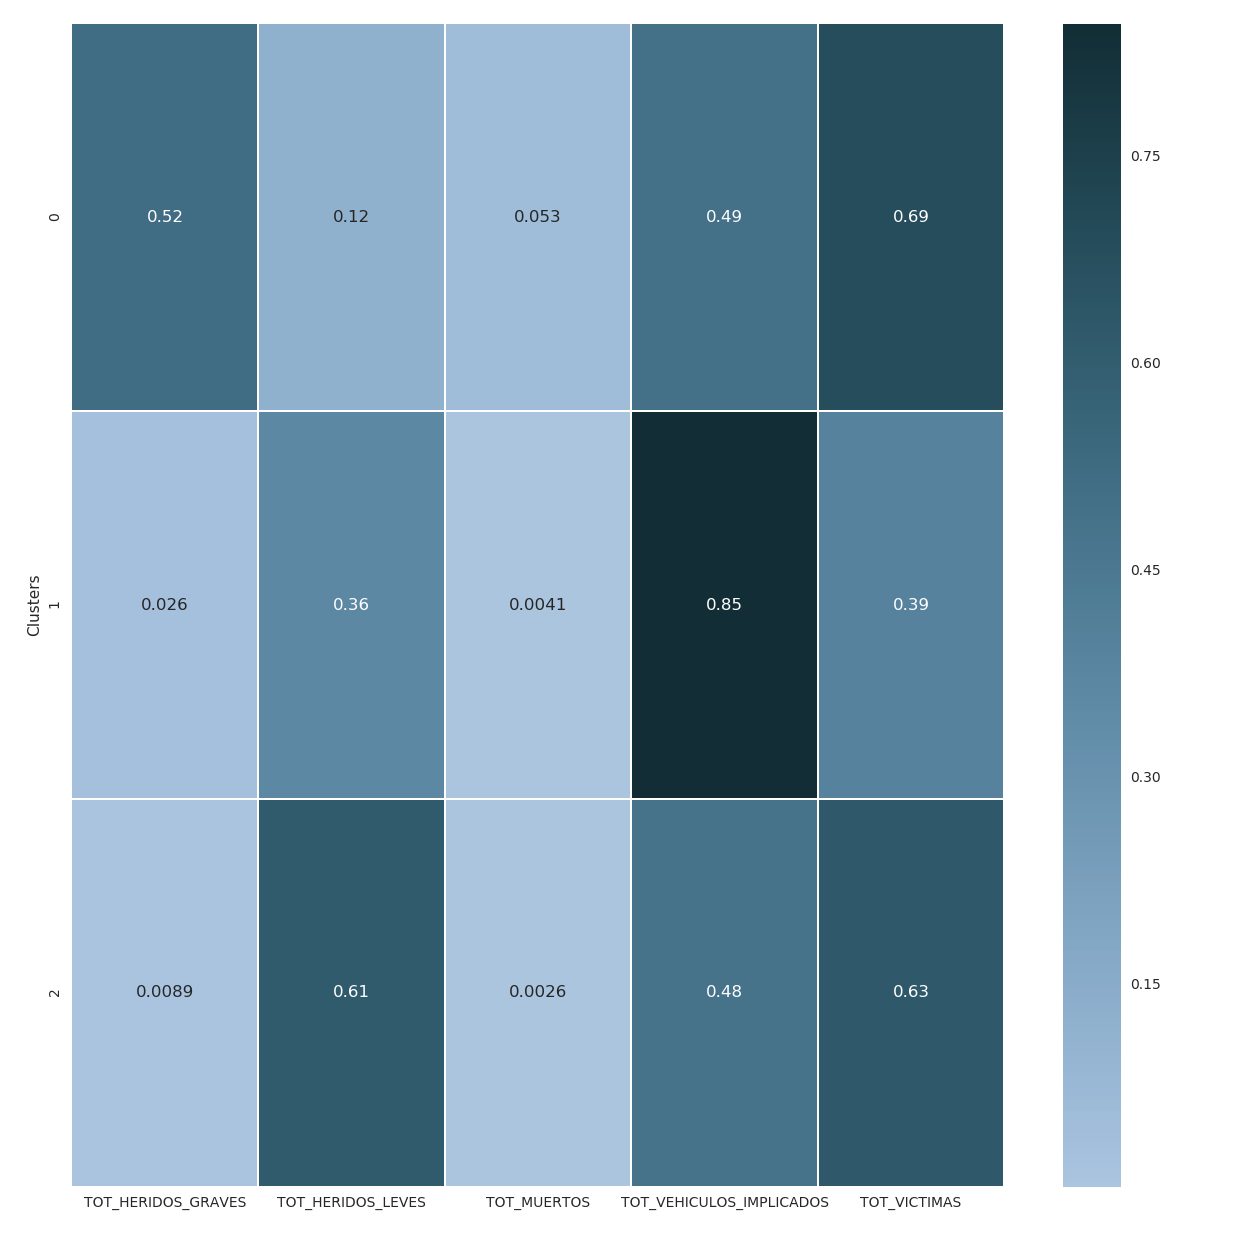
\includegraphics[scale=0.4]{heatmaps/Birch-HighwayAccidents-Heatmap.png}
		\caption{Heatmap del algoritmo Birch para el primer caso de estudio.}
	\end{figure}

	\subsection{Interpretación de la segmentación}
	En este apartado se analizarán los resultados obtenidos basándonos en lo que se muestra en las gráficas y se intentará dar la visión más profesional posible de lo que se puede valorar de los datos recogidos.\\
	
	\subsubsection{K-Means}
	Observando la representación de la matriz de confusión, y apoyándonos en los datos de la tabla, se puede interpretar fácilmente a qué tipo de accidente se corresponde cada cluster. El cluster 0 y el cluster 2 son muy parecidos, siendo ambos accidentes donde no hay muchas víctimas graves ni fallecidos, pero sin embargo hay una gran cantidad de heridos leves, por lo que su total de víctimas asciende considerablemente. En particular, el cluster 0 recoge mayormente aquellos accidentes en los que habiendo menos vehículos se han producido más víctimas, presumiblemente por un choque más fuerte entre dos vehículos, mientras que el cluster 2 recoge los accidentes con más implicados y algo menos de víctimas. Estos datos, aparte de con la tabla de valores medios, pueden verse claramente reflejados en el heatmap del algoritmo, con la leyenda de color señalando dónde hay más víctimas y heridos leves. Adicionalmente, en la matriz de dispersión, se puede observar muy bien lo parecidos que son ambos clusters, y sin embargo cómo se pueden diferenciar, en alguna gráfica como la que representa el total de víctimas frente al total de heridos leves.\\
	
	Como la contraparte a estos dos clusters, el cluster 3 es posiblemente el más devastador, ya que representa accidentes que han tenido también bastantes víctimas pero estas han resultado heridas gravemente o han fallecido. En la matriz de dispersión puede observarse, en la intersección entre la fila y la columna que representan el total de muertos, que sin embargo hay bastantes ejemplos de este cluster que no representan accidentes mortales. No obstante, en la gráfica se aprecia que la mayor parte de todos los demás accidentes que han causado algún muerto están en el cluster 3. Además, esa misma gráfica revela un dato que teníamos como objeto de nuestro estudio: \textbf{los accidentes que suceden en autovías y autopistas no suponen víctimas mortales en la mayoría de los casos.}\\
	
	Por último, el cluster 1 representa los accidentes menos graves, con pocas víctimas y muchos vehículos implicados, como el clásico choque en cadena donde varios conductores pueden sufrir un latigazo cervical sin resultar en más complicaciones ni secuelas. Esto se puede observar de la mejor forma en la gráfica de la matriz de dispersión que representa el total de víctimas frente al total de vehículos implicados. Casi todos los accidentes en los que intervienen más de 2 ó 3 vehículos se reúnen entre el cluster 1 y el 3, sin embargo la gran diferencia existente entre ambos clusters reside en el número de víctimas, donde además en el cluster 3 la mayoría son graves. La representación en el heatmap de ambos clusters refuerza esta posición y la caracterización de estos clusters de dicha forma.
	
	\subsubsection{Birch}
	A diferencia de los clusters en los que se ha dividido anteriormente el algoritmo K-Means, este algoritmo ha reducido el número de clusters y representa esencialmente lo mismo en 3. El cluster 0 del algoritmo Birch es muy similar al agrupamiento que se encuentra en el cluster 3 del K-Means, el que tiene mayor cantidad de muertos y heridos graves. Tanto en la tabla de medias como en el heatmap se puede observar que este cluster es el que contiene los accidentes más graves, y con pocos vehículos implicados, por lo que entendemos que generalmente se trata de colisiones entre dos vehículos o de colisión frontolateral de algún vehículo con una mediana, y que generalmente han debido ser a gran velocidad para causar un impacto tan grande.\\
	
	No obstante, dicho cluster no supone una gran representación dentro del algoritmo. Si se observa la matriz de confusión de Birch se puede apreciar en distintas gráficas, entre ellas cualquiera en la que a raíz de los datos anteriores vayamos a saber que aparece este cluster, como la que representa total de muertos con el total de víctimas, que el número de puntos de la nube de puntos de la gráfica correspondientes al cluster 0 es escaso. Esto quiere decir que, o los datos están muy juntos (son muy similares), o el número de ejemplos de dicha clase es muy pequeño. A juzgar por los valores tan pequeños que tiene toda la columna de medias de muertos en el heatmap, y que el resto de clusters aparecen con una cantidad de puntos mucho mayor en cada una de las demás gráficas, considero que es un cluster que constituye pocos ejemplos.\\
	
	Es destacable que algo similar a lo que ocurre con el cluster 0 y el cluster 3 de K-Means ocurre con los clusters 1 y 2; el cluster 1 de Birch es casi un calco del cluster 1 de K-Means, y el cluster 2 de Birch lo es del cluster 0 de K-Means.\\
	
	La mejor forma de interpretar este hecho es que Birch prácticamente ha rehecho las agrupaciones de K-Means, con unas pequeñas fluctuaciones en los valores medios de cada variable debido a los cambios de asignaciones a cluster que pueda haber en las fronteras. Como podíamos observar en la tabla de resultados de los algoritmos (tabla \ref{tablaTodos1}), Birch deja un cluster sin validez al tener menos del 1\% de los datos, y este podría ser el equivalente al cluster 2 de K-Means, que era similar al cluster 0 pero con unas varianzas mayores en términos de total de vehículos implicados y de víctimas.\\
	
	Los ejemplos de Birch por tanto están clasificados siguiendo el mismo esquema que en el caso anterior, pero reducidos a un total de 3 clusters. Por la mayor diversidad que ofrece K-Means al repartir mejor sus ejemplos y por sus mejores métricas tanto Calinski-Harabaz como Silhouette, creo que es el que mejor solución obtiene de los dos, y casi aún más importante, en el que más visual e interpretativo resulta su análisis.
	
	\subsection{Otras configuraciones de parámetros}
	En este apartado final se ejecutarán los algoritmos con distintas configuraciones de parámetros y se tratarán de elevar sus métricas Calinski-Harabaz y Silhouette para que ver cuáles agrupan mejor los ejemplos según estos criterios.
	
	\subsubsection{K-Means}
	
	Para el algoritmo K-Means se han aumentado el número de clusters de 1 en 1, entre 4 y 9. Los resultados son los que se muestran en la siguiente tabla.
	
	\begin{table}[H]
		\centering
		\resizebox{\textwidth}{!}{
			$\begin{tabular}{ *{7}{c} }
			\toprule
			\textbf{Clusters} & \textbf{Execution time} & \textbf{CH Score} & \textbf{Silhouette Score} & \textbf{Clusters after filtering} & \textbf{Number of samples dropped}\\
			\midrule
			4 & 0.056 & 17443.397 & 0.74487 & 4 & 0 \\
			5 & 0.052 & 18871.057 & 0.74880 & 5 & 0 \\
			6 & 0.052 & 20219.448 & 0.78829 & 6 & 0 \\
			7 & 0.054 & 25698.248 & 0.81488 & 7 & 0 \\
			8 & 0.064 & 24465.708 & 0.84153 & 8 & 0 \\
			9 & 0.068 & 30473.332 & 0.86364 & 9 & 0 \\
			\bottomrule
			\end{tabular}$
		}
		\caption{Configuración de parámetros del algoritmo K-Means en el primer caso de estudio.}
	\end{table}
	
	Como puede observarse, ambas métricas crecen sustancialmente cuando se aumenta el número de clusters. Además, debido al comportamiento de K-Means todos los clusters contienen una cantidad consecuente de ejemplos como para no tener que desechar ninguno. Puesto en este contexto, de las configuraciones probadas la que mejor parece funcionar es la que agrupa los ejemplos en \textbf{9 clusters}.
	
	\subsubsection{Birch}
	
	Para el algoritmo Birch se han aumentado primero los clusters de 1 en 1 entre 4 y 6, y a continuación sobre la configuración inicial de 4 clusters se ha aumentado el umbral desde 0.1 hasta 0.3. Los resultados obtenidos aparecen en la siguiente tabla.
	
	\begin{table}[H]
		\centering
		\resizebox{\textwidth}{!}{
			$\begin{tabular}{ *{7}{c} }
			\toprule
			\textbf{Clusters} & \textbf{Threshold} & \textbf{Execution time} & \textbf{CH Score} & \textbf{Silhouette Score} & \textbf{Clusters after filtering} & \textbf{Number of samples dropped}\\
			\midrule
			4 & 0.1 & 0.385 & 10526.549 & 0.67967 & 3 & 91 \\
			5 & 0.1 & 0.380 & 8119.076 & 0.67754 & 3 & 140 \\
			6 & 0.1 & 0.382 & 10682.449 & 0.71477 & 4 & 140 \\
			4 & 0.2 & 0.378 & 13125.399 & 0.70941 & 4 & 0 \\
			4 & 0.3 & 0.376 & 2337.262 & 0.50971 & 4 & 0 \\
			\bottomrule
			\end{tabular}$
		}
		\caption{Configuración de parámetros del algoritmo Birch en el primer caso de estudio.}
	\end{table}
	
	De acuerdo a los experimentos planteados con este algoritmo parece que la mejor configuración, la que presenta un mayor equilibrio, sería la que cuenta con \textbf{4 clusters y un umbral de 0.2}. Además esto provoca que los ejemplos tiendan a agruparse más y no se queden perdidos por el espacio de búsqueda, por lo que se puede ver que no se desprende de ningún ejemplo cuando se da esta configuración, resultando ser sus mejores parámetros de entre los considerados.
	
	\section{Caso de estudio 2}
	
	\subsection{¿Qué se analiza?}
	El segundo caso de estudio que se va a analizar en la práctica tiene como centro de atención los \textbf{accidentes ocurridos de madrugada}, es decir, aquellos que ocurren entre las 0:00 y las 6:00 según el criterio que he seguido. Las características que se van a tener en cuenta son las mismas que en el caso anterior, a saber, número de heridos graves y leves, número total de víctimas, número de vehículos implicados y número de muertos. De nuevo se buscará saber cómo se distribuyen principalmente los accidentes en estas horas, cuántas personas mueren o se hieren de gravedad y si representan un gran número de ejemplos o son casos que se pueden considerar aislados.\\
	
	Este caso de estudio tiene un tamaño medio. Está compuesto por 5969 ejemplos.
	
	\subsection{Resultados de los algoritmos}
	
	A continuación se muestra la tabla de los resultados de los algoritmos para este segundo caso de estudio. Como en el primer apartado, esta tabla incluirá las puntuaciones de los algoritmos según las métricas Calinski-Harabaz y Silhouette, además de los clusters en los que ha dividido los ejemplos y su tiempo de ejecución. Adicionalmente, se ha optado también por filtrar aquellos clusters que no agrupen un 1\% de los datos para que los heatmaps y tablas de medias no contengan outliers y puedan ser así más lógicos y sencillos de interpretar.
	
	\begin{table}[H]
		\centering
		\resizebox{\textwidth}{!}{
			$\begin{tabular}{ *{7}{c} }
			\toprule
			\textbf{Algorithm} & \textbf{Clusters} & \textbf{Execution time} & \textbf{CH Score} & \textbf{Silhouette Score} & \textbf{Clusters after filtering} & \textbf{Number of samples dropped}\\
			\midrule
			K-Means & 4 & 0.022 & 8773.443 & 0.78234 & 4 & 0 \\
			DBSCAN & 22 & 0.268 & 2218.602 & 0.72603 & 8 & 255 \\
			Birch & 4 & 0.183 & 4435.925 & 0.70089 & 3 & 1 \\
			Spectral Clustering & 4 & 6.952 & 7897.146 & 0.74936 & 4 & 0 \\
			Ward & 100 & 0.625 & - & - & 9 & 587 \\
			\bottomrule
			\end{tabular}$
		}
		\caption{Resultados de los algoritmos de clustering para el segundo caso de estudio.}
	\end{table}

	En este caso los resultados de los scores vuelven a ser muy similares al primer caso de estudio, pero como ya hemos trabajado con K-Means, en esta ocasión lo haremos con \textbf{Spectral Clustering}. Además, para esta ocasión contaremos también con un análisis del algoritmo \textbf{Ward}, un algoritmo de clustering jerárquico aglomerativo que genera una gran cantidad de clusters (tantos como individuos haya en la población) y los va uniendo dos a dos en cada paso, para acabar obteniendo el número de clusters indicado como parámetro. A pesar de tener un montón de clusters inicialmente (100, los indicados en el código como parámetro) estos se ven reducidos cuando se aplica el filtrado del 1\%, por lo que trabajar con 9 clusters es ya más manejable. Estos dos algoritmos serán el objeto de estudio para este caso.
	
	\subsubsection{Spectral Clustering}
	En primer lugar se muestra la matriz de dispersión del algoritmo Spectral Clustering para el segundo caso de estudio.
	
	\begin{figure}[H]
		\centering
		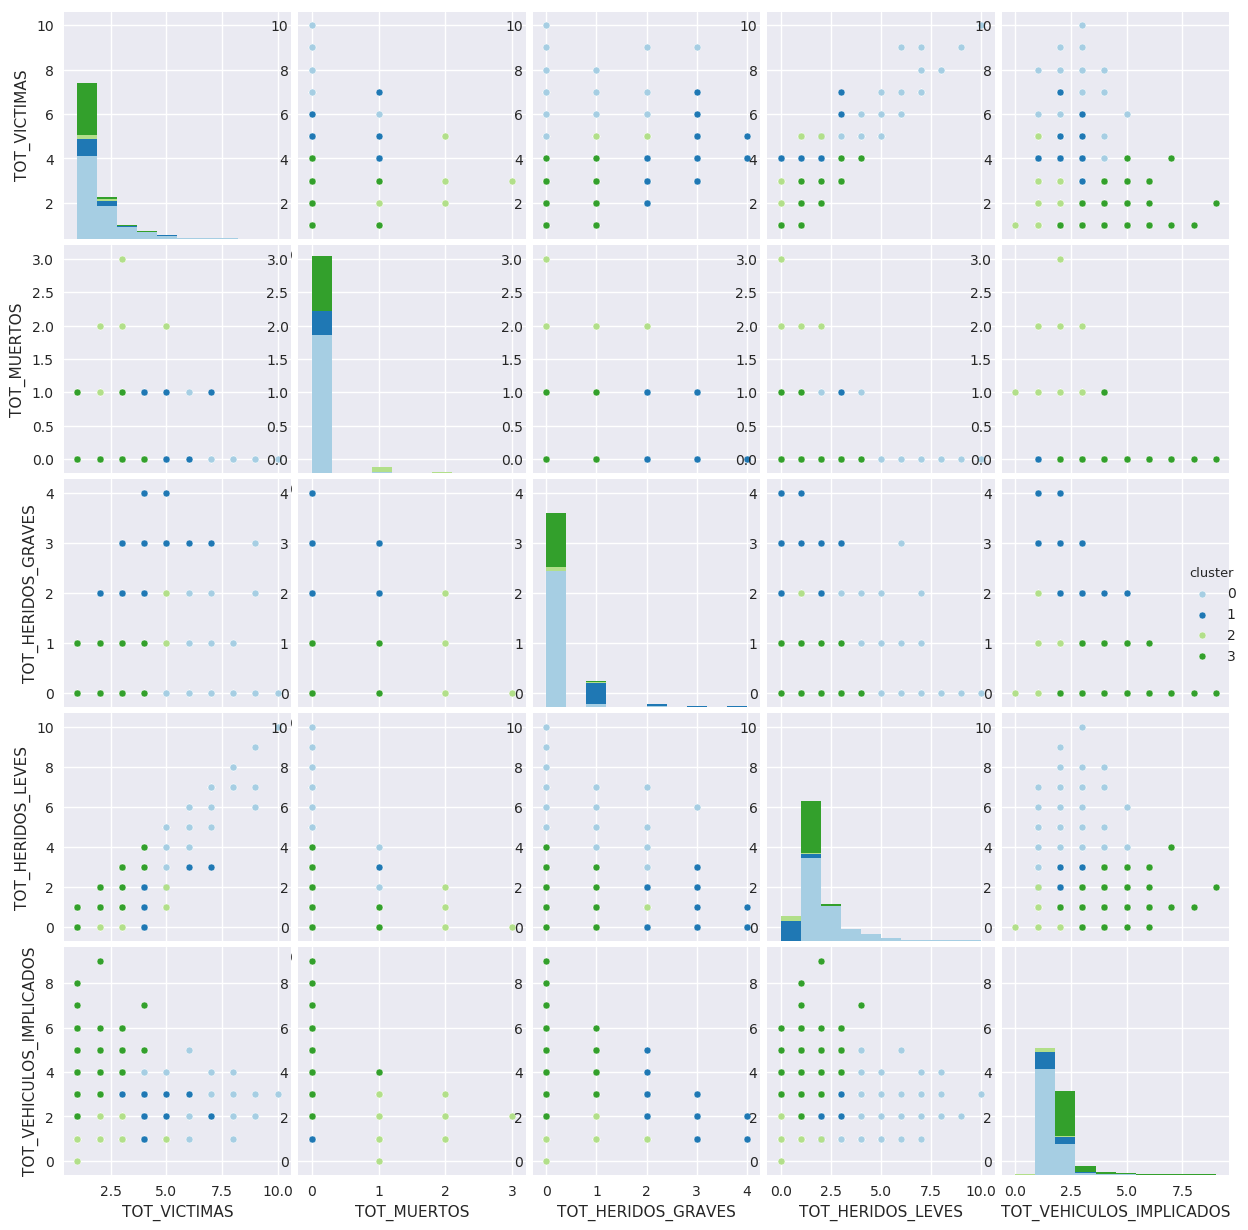
\includegraphics[scale=0.5]{plots/SpectralClustering-EarlyMorningAccidents-ScatterMatrix.png}
		\caption{Matriz de dispersión del algoritmo Spectral Clustering para el segundo caso de estudio.}
	\end{figure}
	
	Ahora se muestra la tabla de medias por variable para cada cluster para este algoritmo.
	
	\begin{table}[H]
		\centering
		\resizebox{\textwidth}{!}{
			\begin{tabular}{*{6}{c}}
				\toprule
				\textbf{CLUSTER} &  \textbf{TOT\_HERIDOS\_GRAVES} &  \textbf{TOT\_HERIDOS\_LEVES} &  \textbf{TOT\_MUERTOS} &  \textbf{TOT\_VEHICULOS\_IMPLICADOS} &  \textbf{TOT\_VICTIMAS} \\
				\midrule
				\textbf{0} &            0.023976 &           1.677263 &     0.002963 &                  1.254849 &      1.704203 \\
				\textbf{1} &            1.160686 &           0.198128 &     0.012480 &                  1.332293 &      1.371295 \\
				\textbf{2} &            0.170068 &           0.156463 &     1.081633 &                  1.326531 &      1.408163 \\
				\textbf{3} &            0.016338 &           1.044929 &     0.001361 &                  2.282505 &      1.062628 \\
				\bottomrule
			\end{tabular}
		}
		\caption{Tabla de valores medios del algoritmo Spectral Clustering para el segundo caso de estudio.}
	\end{table}
	
	Se puede observar por último el heatmap correspondiente a los valores normalizados del caso anterior para el mismo algoritmo y cada uno de sus clusters.
	
	\begin{figure}[H]
		\centering
		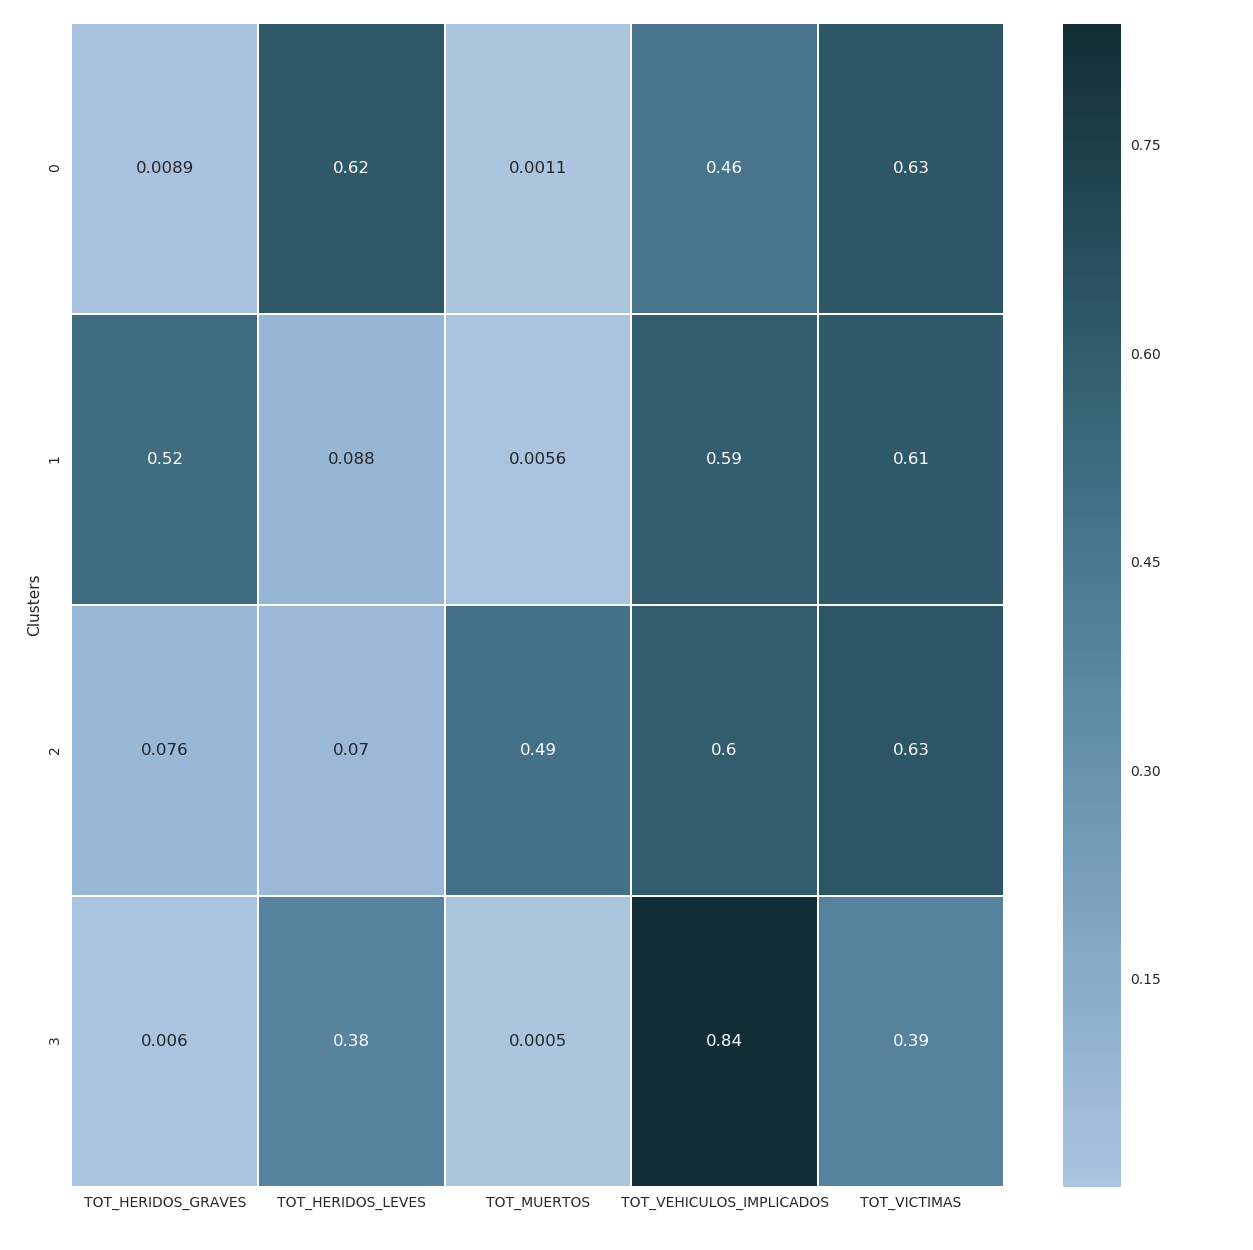
\includegraphics[scale=0.4]{heatmaps/SpectralClustering-EarlyMorningAccidents-Heatmap.png}
		\caption{Heatmap del algoritmo Spectral Clustering para el segundo caso de estudio.}
	\end{figure}
	
	\subsubsection{Ward}
	Se muestra a continuación la matriz de dispersión del algoritmo Ward para el segundo caso de estudio, ya con el filtrado de clusters aplicado. A pesar de que la gráfica más importante para el algoritmo Ward se muestra un poco más adelante, ya que existe la posibilidad se muestra también esta matriz de dispersión por si se considera adecuado o interesante comparar los resultados obtenidos con la distribución de los ejemplos en función de las distintas variables.
	
	\begin{figure}[H]
		\centering
		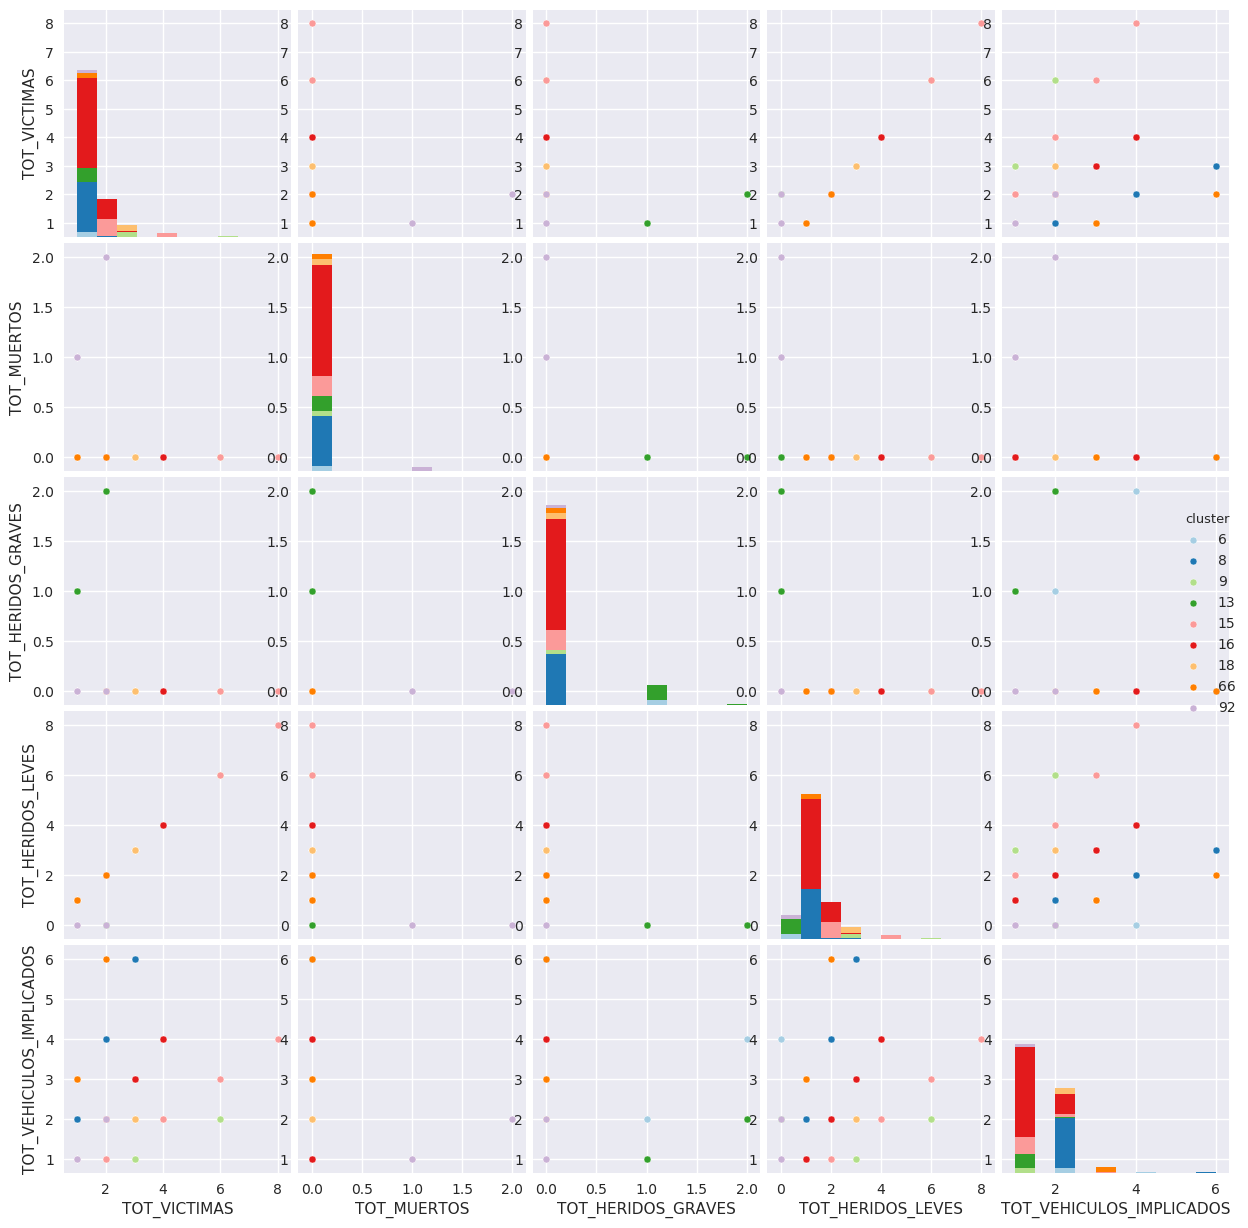
\includegraphics[scale=0.5]{plots/Ward-EarlyMorningAccidents-ScatterMatrix.png}
		\caption{Matriz de dispersión del algoritmo Ward para el segundo caso de estudio.}
	\end{figure}
	
	A continuación se puede ver la tabla de valores medios por cada variable y cluster que ha agrupado el algoritmo Ward.
	
	\begin{table}[H]
	\centering
	\resizebox{\textwidth}{!}{
		\begin{tabular}{*{6}{c}}
			\toprule
			\textbf{CLUSTER} &  \textbf{TOT\_HERIDOS\_GRAVES} &  \textbf{TOT\_HERIDOS\_LEVES} &  \textbf{TOT\_MUERTOS} &  \textbf{TOT\_VEHICULOS\_IMPLICADOS} &  \textbf{TOT\_VICTIMAS} \\
			\midrule
			\textbf{66} &            0.000000 &           1.008772 &     0.000000 &                  3.026316 &      1.008772 \\
			\textbf{6 } &            1.008475 &           0.000000 &     0.000000 &                  2.016949 &      1.008475 \\
			\textbf{8 } &            0.000000 &           1.013832 &     0.000000 &                  2.027665 &      1.013832 \\
			\textbf{9 } &            0.000000 &           3.176471 &     0.000000 &                  1.058824 &      3.176471 \\
			\textbf{13} &            1.040761 &           0.000000 &     0.000000 &                  1.040761 &      1.040761 \\
			\textbf{15} &            0.000000 &           2.358025 &     0.000000 &                  1.179012 &      2.358025 \\
			\textbf{16} &            0.000000 &           1.196324 &     0.000000 &                  1.196324 &      1.196324 \\
			\textbf{18} &            0.000000 &           3.000000 &     0.000000 &                  2.000000 &      3.000000 \\
			\textbf{92} &            0.000000 &           0.000000 &     1.012346 &                  1.012346 &      1.012346 \\
			\bottomrule
		\end{tabular}
	}
	\caption{Tabla de valores medios del algoritmo Ward para el segundo caso de estudio.}
	\end{table}
	
	Para el algoritmo Ward, al ser un algoritmo jerárquico, se ha construido un dendrograma para analizar la similitud de sus clusters resultantes y cómo se agrupan. Este dendrograma aparece junto al heatmap, y se ha calculado utilizando el método ``clustermap'' del paquete \textit{seaborn}. Esta será la gráfica principal en la que centraremos nuestro estudio del algoritmo, ya que seguramente es la que más interpretabilidad tiene para un algoritmo jerárquico.
	
	\begin{figure}[H]
		\centering
		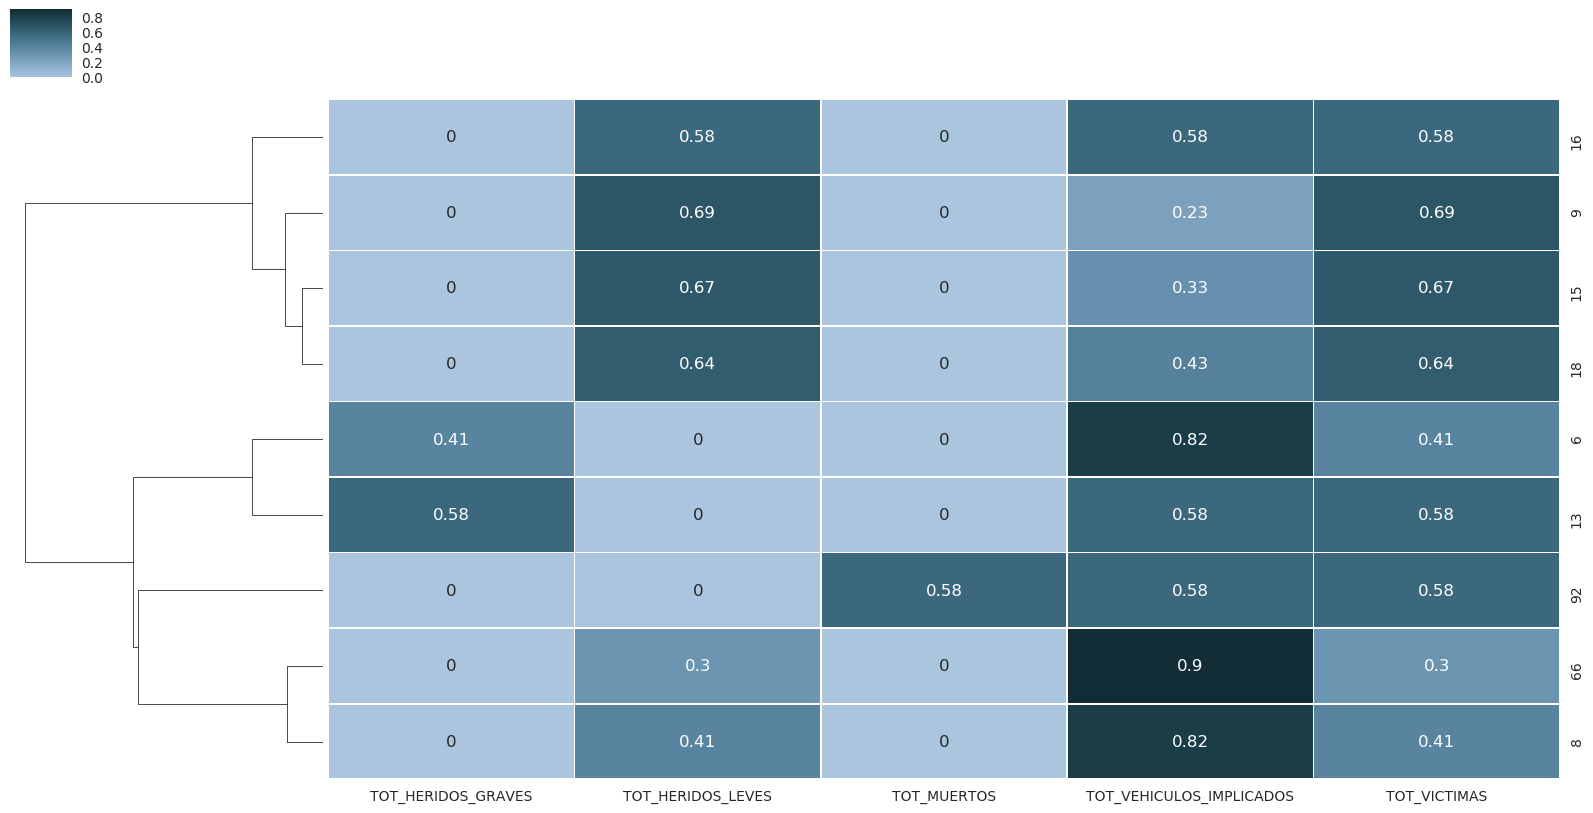
\includegraphics[scale=0.4]{dendrograms/Ward-EarlyMorningAccidents-Dendrogram.png}
		\caption{Dendrograma del algoritmo Ward junto a su heatmap para el segundo caso de estudio.}
	\end{figure}
	
	\subsection{Interpretación de la segmentación}
	En este apartado final del segundo caso de estudio se realizará una interpretación del contenido de los distintos clusters que cada algoritmo ha agrupado y se intentará dar una visión acertada de los rasgos que caracterizan a cada uno de ellos. Para ello se hará uso de las gráficas y tablas expuestas en el apartado anterior.
	
	\subsubsection{Spectral Clustering}
	Spectral Clustering es el segundo algoritmo que mejor métricas de Calinski-Harabaz y Silhouette obtiene, solo por detrás de K-Means, y ambos no tienen necesidad de filtrar ningún cluster. Esto nos indica que los clusters que agrupa Spectral Clustering no tienen en general baja representación y que cada uno de ellos merece ser tenido en cuenta.\\
	
	Lo primero que llama la atención de este caso de estudio es que la gran mayoría de víctimas mortales se reúnen en uno de los clusters, de ahí la gran diferencia de color en el heatmap del cluster 2 en la columna de muertes con respecto al resto de clusters. También es destacable que este algoritmo para este caso de estudio es capaz de dividir los ejemplos de forma que en el cluster 2 queden aquellos accidentes mortales en los que apenas hay heridos graves ni leves (las víctimas casi en su totalidad fallecen) y sin embargo en el cluster 1 se agrupen los que tienen heridos graves pero apenas fallecidos. Es un comportamiento llamativo del caso de estudio, en el que parece que no hay punto medio a la hora de hacer el recuento de víctimas.\\
	
	Si observamos la matriz de dispersión se puede apreciar que sí que existen casos de muerte en cada uno de los clusters (en la representación de total de muertos contra total de heridos leves por ejemplo), sin embargo sí es cierto que para el resto de clusters la cantidad de fallecimientos es bastante inferior al de este cluster en cuestión.\\

	El resto de clusters siguen una agrupación natural, y básicamente similar a la que encontrábamos en otros ejemplos anteriores, pues la distribución de los accidentes resulta ser similar; existe un cluster para aquellos accidentes graves con varios heridos graves pero pocos o ningún fallecido, y dos para accidentes con heridos leves, uno de ellos con más vehículos implicados y pocas víctimas (el caso del choque en cadena indicado anteriormente) y otro con menos vehículos y más heridos leves, y por consecuente más víctimas.\\
	
	La agrupación de este algoritmo es bastante buena y sigue unos criterios bastante lógicos para distinguir unos accidentes de otros. Al contar con solo 4 clusters los accidentes están suficientemente bien definidos pero no el algoritmo no tiene necesidad de entrar a valorar casos muy particulares, y se ve reflejado positivamente en las métricas y en la interpretabilidad de la matriz de dispersión y del heatmap.
	
	\subsubsection{Ward}
	Como se ha indicado antes, para este algoritmo tendrá especial importancia la interpretación del dendrograma, ya que es interesante apreciar cómo se parecen unos clusters a otros para valorar cómo habría sido el resultado esperado de haber fijado menos clusters como parámetro. Para seguir este criterio sólo habría que observar el dendrograma y considerar que el siguiente paso que habría dado el algoritmo habría sido alguna de las uniones entre dos clusters o conjuntos de clusters. Por ejemplo, en este caso el siguiente paso podría haber sido la agrupación de los clusters 6 y 13, que son dos subconjuntos de accidentes donde solamente ha habido heridos graves, aunque en menor y mayor magnitud, respectivamente.\\
	
	De la misma forma ocurre un par de filas por encima en el dendrograma con los clusters 15 y 18, que además tienen valores prácticamente similares en todas las variables, por lo que es también bastante probable que en un paso más del algoritmo hubiesen sido los dos clusters que hubiesen convergido. El dendrograma resulta muy útil para apreciar estas agrupaciones dos a dos, y valorar cómo de bien se comporta el algoritmo con un determinado parámetro ``k'' pasado como argumento.\\
	
	Con respecto a ese tema, para este caso de estudio en particular podemos observar que agrupando los clusters dos a dos y quedándonos con 4 con las uniones que nos sugiere el dendrograma, el heatmap sería muy parecido al del Spectral Clustering o alguno de los algoritmos que hemos visto anteriormente. En esencia, consistiría en unir los clusters 6 y 13, los clusters 8 y 66 (contienen accidentes con muchos vehículos implicados y una cantidad moderada de heridos, todos leves), los clusters 15 y 18, y luego estos a su vez con el cluster 9, con el que comparten similitud en la mayoría de variables. El resultado nos dejaría con 4 clusters que serían capaces de equipararse a los resultantes según el algoritmo anterior.\\
	
	Con esto podemos presumiblemente afirmar que el algoritmo Ward, con un valor de ``k'' adecuado, puede converger hasta obtener clusters como si fuese un algoritmo no-jerárquico. El resto de clusters sobre los que no hemos incidido también tienen distribuciones de accidentes similares a las de casos anteriores: accidentes con muertos y ninguna persona herida, accidentes con solo heridos graves, accidentes con solo heridos leves... Tener tanta variedad de clusters permite prácticamente excluir los distintos valores de las variables y relegarlas a un único cluster.\\
	
	Como nota curiosa, el último dato a tener en cuenta es que si observamos tanto la tabla de medias como el heatmap junto al dendrograma podemos observar que algunos clusters tienen una relación directa entre algunas de sus variables. Por ejemplo, el cluster 16 tiene el mismo valor medio de vehículos implicados como de heridos leves como de víctimas. Sabiendo que los algoritmos de clustering agrupan por similitud de los ejemplos, estoy bastante seguro de que en todos los ejemplos de este cluster tienen un accidente el mismo número de vehículos que de víctimas de carácter leve. La misma situación se puede dar para el caso del cluster 92, con el mismo número de fallecidos que de vehículos implicados. Ambos casos se pueden confirmar si observamos las gráficas correspondientes a la intersección de las columnas/filas de dichas variables en la matriz de dispersión, y se demuestra que estos clusters siguen una distribución lineal.

	\subsection{Otras configuraciones de parámetros}
	Para este apartado solo evaluaremos distintas configuraciones de parámetros del algoritmo Spectral Clustering, ya que solo vamos a basarnos en las puntuaciones de las métricas Calinski-Harabaz y Silhouette y sobre el algoritmo Ward no se han calculado como se ha explicado anteriormente.

	\subsubsection{Spectral Clustering}

	Para el algoritmo Spectral Clustering se han aumentado el número de clusters de 1 en 1, entre 4 y 9, al igual que se hizo anteriormente con el algoritmo K-Means. Los resultados se muestran en la siguiente tabla.

	\begin{table}[H]
		\centering
		\resizebox{\textwidth}{!}{
			$\begin{tabular}{ *{7}{c} }
			\toprule
			\textbf{Clusters} & \textbf{Execution time} & \textbf{CH Score} & \textbf{Silhouette Score} & \textbf{Clusters after filtering} & \textbf{Number of samples dropped}\\
			\midrule
			4 & 6.891 & 7897.146 & 0.74936 & 4 & 0 \\
			5 & 7.805 & 11709.279 & 0.81751 & 5 & 0 \\
			6 & 8.110 & 11616.571 & 0.82454 & 6 & 0 \\
			7 & 8.634 & 15002.242 & 0.85225 & 7 & 0 \\
			8 & 8.990 & 13214.457 & 0.85611 & 7 & 43 \\
			9 & 8.948 & 13759.211 & 0.87439 & 8 & 46 \\
			\bottomrule
			\end{tabular}$
		}
		\caption{Configuración de parámetros del algoritmo Spectral Clustering en el segundo caso de estudio.}
	\end{table}

	Con los valores de ambas métricas que se observan en la tabla y el número de ejemplos que empieza a dejar de considerar a partir de los 8 clusters, considero la mejor configuración la que cuenta con \textbf{7 clusters}, que obtiene la mejor medida en Calinski-Harabaz y casi la mejor en Silhouette.

	\section{Caso de estudio 3}
	
	\subsection{¿Qué se analiza?}
	El tercer y último caso de estudio que se llevará a cabo en la práctica comprende aquellos \textbf{accidentes que han ocurrido en Andalucía, con una calzada que se registró como mojada, y donde el tipo de accidente supuso un vuelco}. Las características a analizar son las mismas de los dos casos de estudio anteriores, número de víctimas, víctimas mortales, heridos graves y leves y número de vehículos implicados. Para este caso tan particular se quiere comprobar sobre todo el comportamiento de un algoritmo jerárquico, para ver qué clusters es capaz de agrupar con un subconjunto tan específico. Es por eso que se ha decidido usar un caso de estudio tan característico y refinado que no representase muchos ejemplos para su correcto estudio según este criterio.\\
	
	Como es de esperar este es el caso de estudio más reducido de todos, con un total de tan solo 78 ejemplos.
	
	\subsection{Resultados de los algoritmos}
	
	A continuación se muestra la tabla de resultados de los distintos algoritmos sobre el subconjunto de datos que representa este caso de estudio. Sobre ella se representan las métricas Calinski-Harabaz y Silhouette, el tiempo de ejecución y los clusters que el algoritmo ha agrupado, junto al número de clusters restantes tras el filtrado y el número de ejemplos que ha eliminado con el mismo.
	
	\begin{table}[H]
		\centering
		\resizebox{\textwidth}{!}{
			$\begin{tabular}{ *{7}{c} }
			\toprule
			\textbf{Algorithm} & \textbf{Clusters} & \textbf{Execution time} & \textbf{CH Score} & \textbf{Silhouette Score} & \textbf{Clusters after filtering} & \textbf{Number of samples dropped}\\
			\midrule
			K-Means & 4 & 0.022 & 530.129 & 0.83994 & 4 & 0 \\
			DBSCAN & 5 & 0.001 & 301.505 & 0.71429 & 5 & 0 \\
			Birch & 4 & 0.003 & 354.076 & 0.83994 & 3 & 1 \\			
			Spectral Clustering & 4 & 0.020 & 436.408 & 0.58813 & 4 & 0 \\			
			Ward & 39 & 0.001 & - & - & 4 & 35 \\			
			\bottomrule
			\end{tabular}$
		}
		\caption{Resultados de los algoritmos de clustering para el tercer caso de estudio.}
	\end{table}

	En este problema con tan pocos datos, como se ha dicho anteriormente es interesante trabajar con un algoritmo jerárquico como \textbf{Ward} otra vez. Además, para utilizar todos los algoritmos en profundidad al menos una vez, se usará el algoritmo \textbf{DBSCAN} para complementar el análisis. El algoritmo Ward en este caso deja fuera del estudio 35 datos que considera outliers por pertenecer a clusters con un solo ejemplo.\\
	
	Cabe destacar que se ha introducido un comportamiento particular sobre el número de clusters que debe obtener el algoritmo Ward, y es que este es 100 siempre y cuando ese valor no esté por encima del 50\% del tamaño total del conjunto de datos. En caso de ser así, Ward pasa a hacer tantos clusters como resulten ser la mitad de ejemplos del conjunto. En este caso, ha hecho 39 clusters, la mitad de los 78 ejemplos de los que se componía el caso de estudio.
	
	\subsubsection{DBSCAN}
	
	En primer lugar se muestra la matriz de dispersión del algoritmo DBSCAN.
	
	\begin{figure}[H]
		\centering
		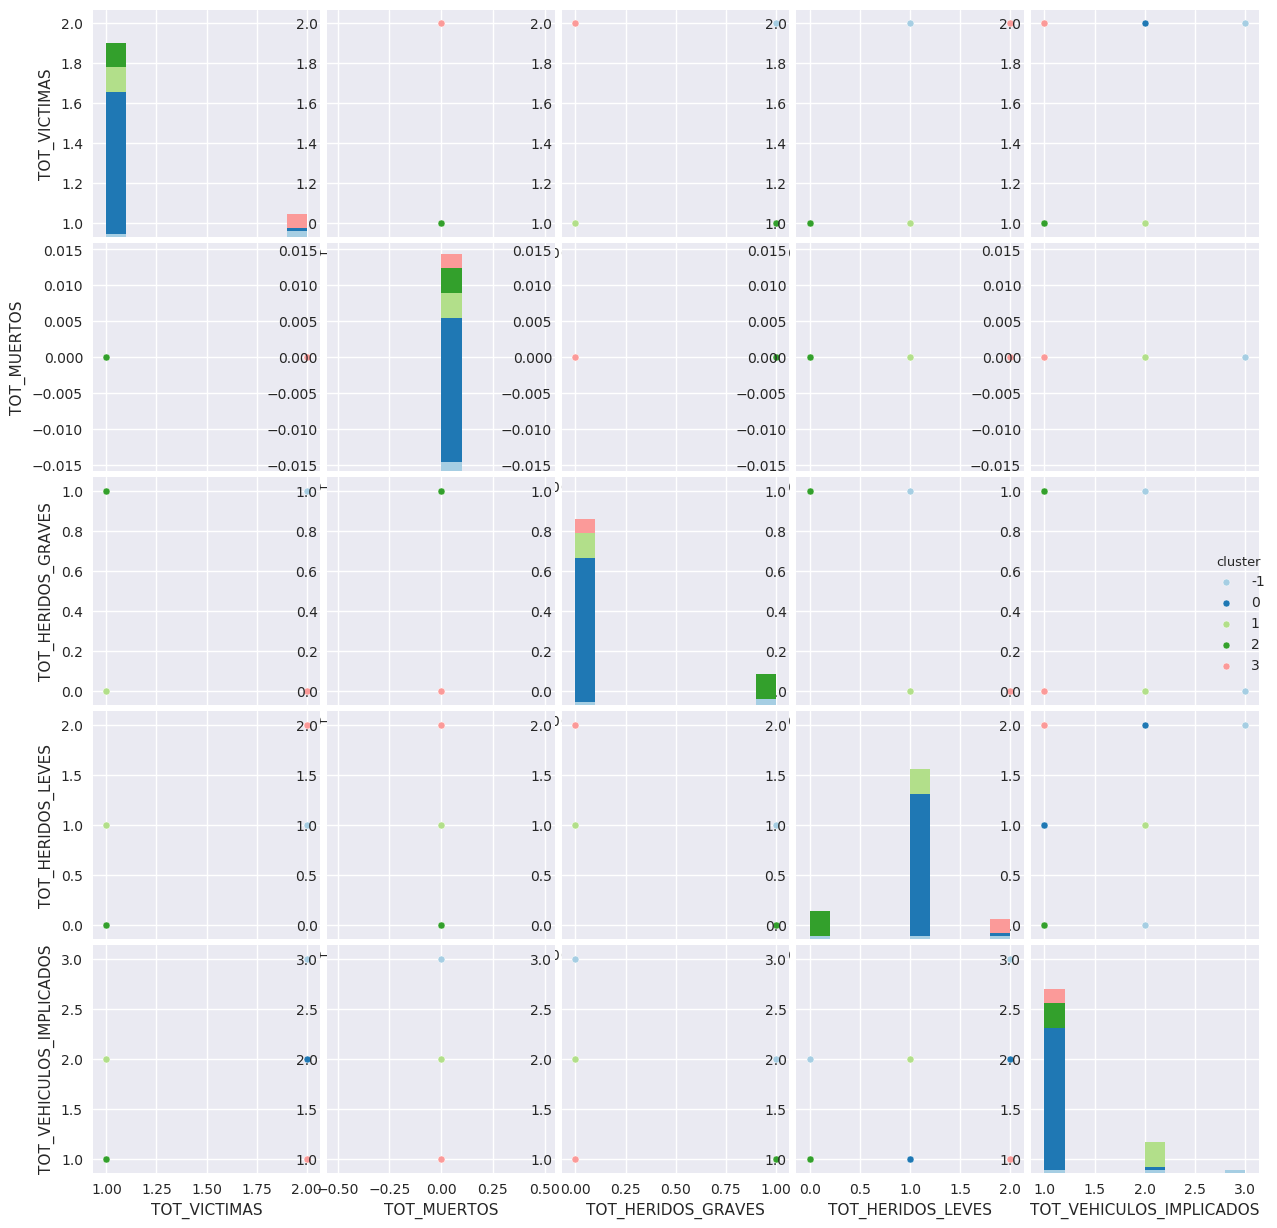
\includegraphics[scale=0.5]{plots/DBSCAN-WetOverturnedAccidents-ScatterMatrix.png}
		\caption{Matriz de dispersión del algoritmo DBSCAN para el tercer caso de estudio.}
	\end{figure}

	Como se puede observar la matriz de dispersión pierde una importante interpretabilidad cuando el conjunto de ejemplos es tan reducido, por lo tanto no merecerá la pena indagar más sobre ella. A pesar de ello la he decidido mostrar para que se vea de primera mano que no es representativa en casos de estudio tan específicos.\\
	
	Ahora se muestra la tabla de valores medios para este caso de estudio.
	
	\begin{table}[H]
		\centering
		\resizebox{\textwidth}{!}{
			\begin{tabular}{*{6}{c}}
				\toprule
				\textbf{CLUSTER} &  \textbf{TOT\_HERIDOS\_GRAVES} &  \textbf{TOT\_HERIDOS\_LEVES} &  \textbf{TOT\_MUERTOS} &  \textbf{TOT\_VEHICULOS\_IMPLICADOS} &  \textbf{TOT\_VICTIMAS} \\
				\midrule
				\textbf{0 } &            0.000000 &           1.019231 &          0.0 &                  1.019231 &      1.019231 \\
				\textbf{1 } &            0.000000 &           1.000000 &          0.0 &                  2.000000 &      1.000000 \\
				\textbf{2 } &            1.000000 &           0.000000 &          0.0 &                  1.000000 &      1.000000 \\
				\textbf{3 } &            0.000000 &           2.000000 &          0.0 &                  1.000000 &      2.000000 \\
				\textbf{-1} &            0.666667 &           1.000000 &          0.0 &                  2.000000 &      1.666667 \\
				\bottomrule
			\end{tabular}
		}
		\caption{Tabla de valores medios del algoritmo DBSCAN para el tercer caso de estudio.}
	\end{table}

	Por último para el algoritmo DBSCAN se muestra su heatmap representando las distintas variables respecto a los clusters.
	
	\begin{figure}[H]
		\centering
		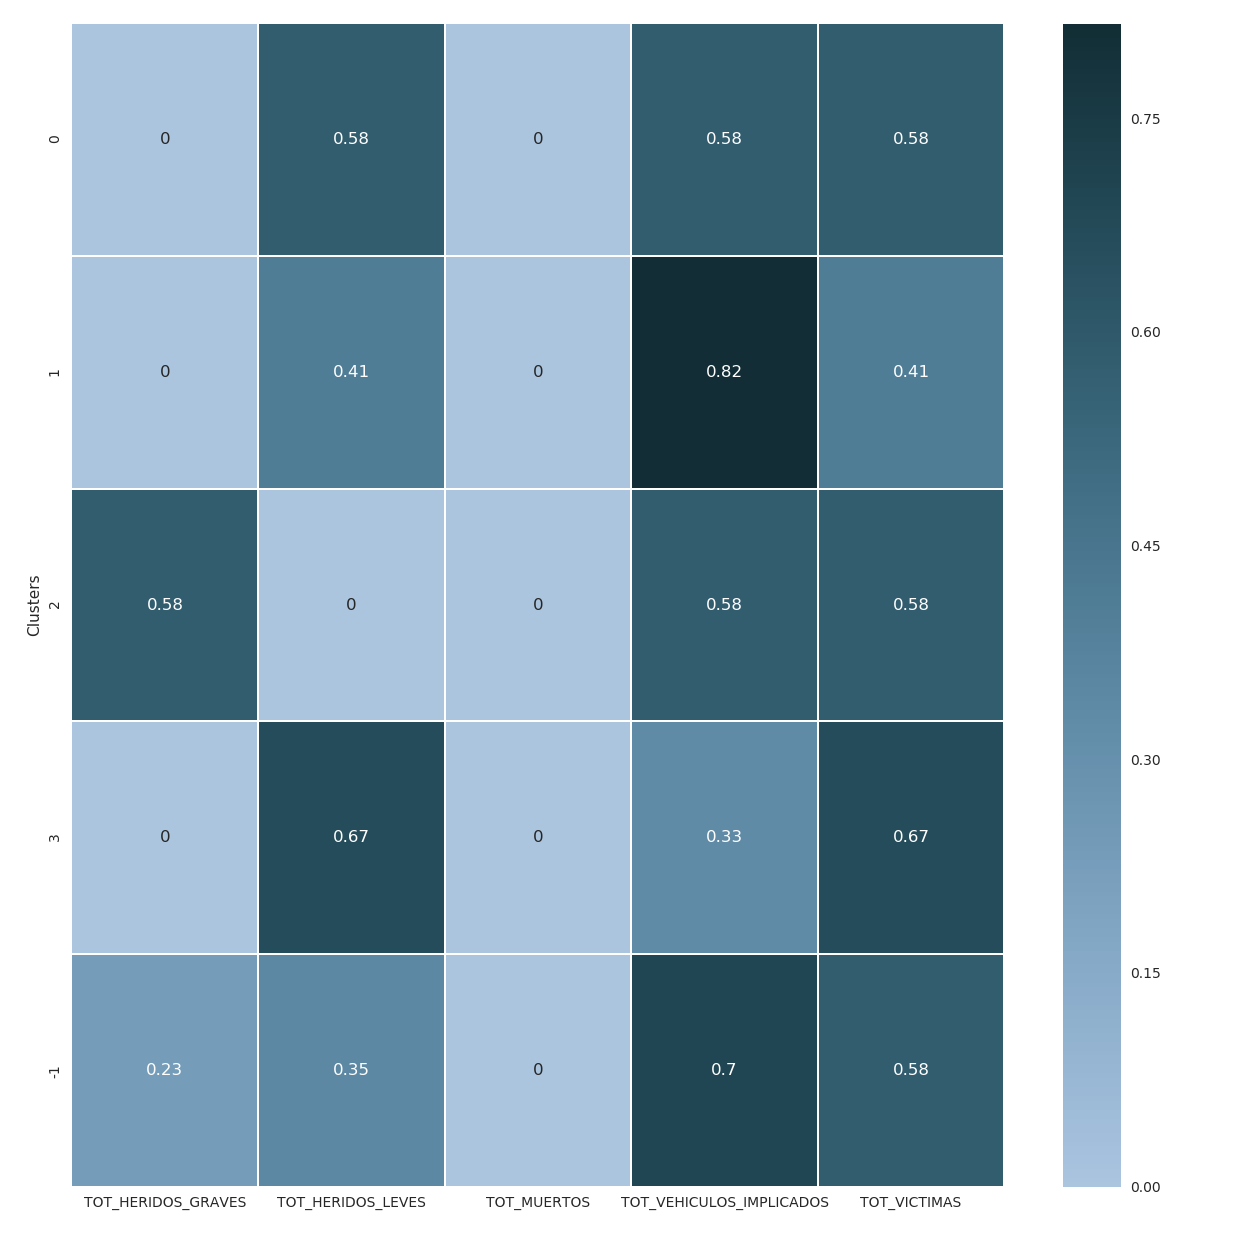
\includegraphics[scale=0.4]{heatmaps/DBSCAN-WetOverturnedAccidents-Heatmap.png}
		\caption{Heatmap del algoritmo DBSCAN para el tercer caso de estudio.}
	\end{figure}

	\subsubsection{Ward}
	
	Para este caso en particular como hemos indicado antes no merece la pena utilizar la matriz de dispersión para nuestro análisis, doblemente en el caso de este algoritmo que es perfectamente interpretable mediante la tabla de valores medios y sobre todo el heatmap y el dendrograma. Por tanto, lo primero en mostrarse será la tabla de medias.
	
	\begin{table}[H]
		\centering
		\resizebox{\textwidth}{!}{
			\begin{tabular}{*{6}{c}}
				\toprule
				\textbf{CLUSTER} &  \textbf{TOT\_HERIDOS\_GRAVES} &  \textbf{TOT\_HERIDOS\_LEVES} &  \textbf{TOT\_MUERTOS} &  \textbf{TOT\_VEHICULOS\_IMPLICADOS} &  \textbf{TOT\_VICTIMAS} \\
				\midrule
				\textbf{0} &                 0.0 &                1.0 &          0.0 &                       1.0 &           1.0 \\
				\textbf{1} &                 0.0 &                2.0 &          0.0 &                       1.0 &           2.0 \\
				\textbf{2} &                 1.0 &                0.0 &          0.0 &                       1.0 &           1.0 \\
				\textbf{3} &                 0.0 &                1.0 &          0.0 &                       2.0 &           1.0 \\
				\bottomrule
			\end{tabular}
		}
		\caption{Tabla de valores medios del algoritmo Ward para el tercer caso de estudio.}
	\end{table}
	
	De nuevo, en lugar de un heatmap aislado podemos obtener un heatmap con dendrograma para el algoritmo Ward, y es el que se muestra a continuación.
	
	\begin{figure}[H]
		\centering
		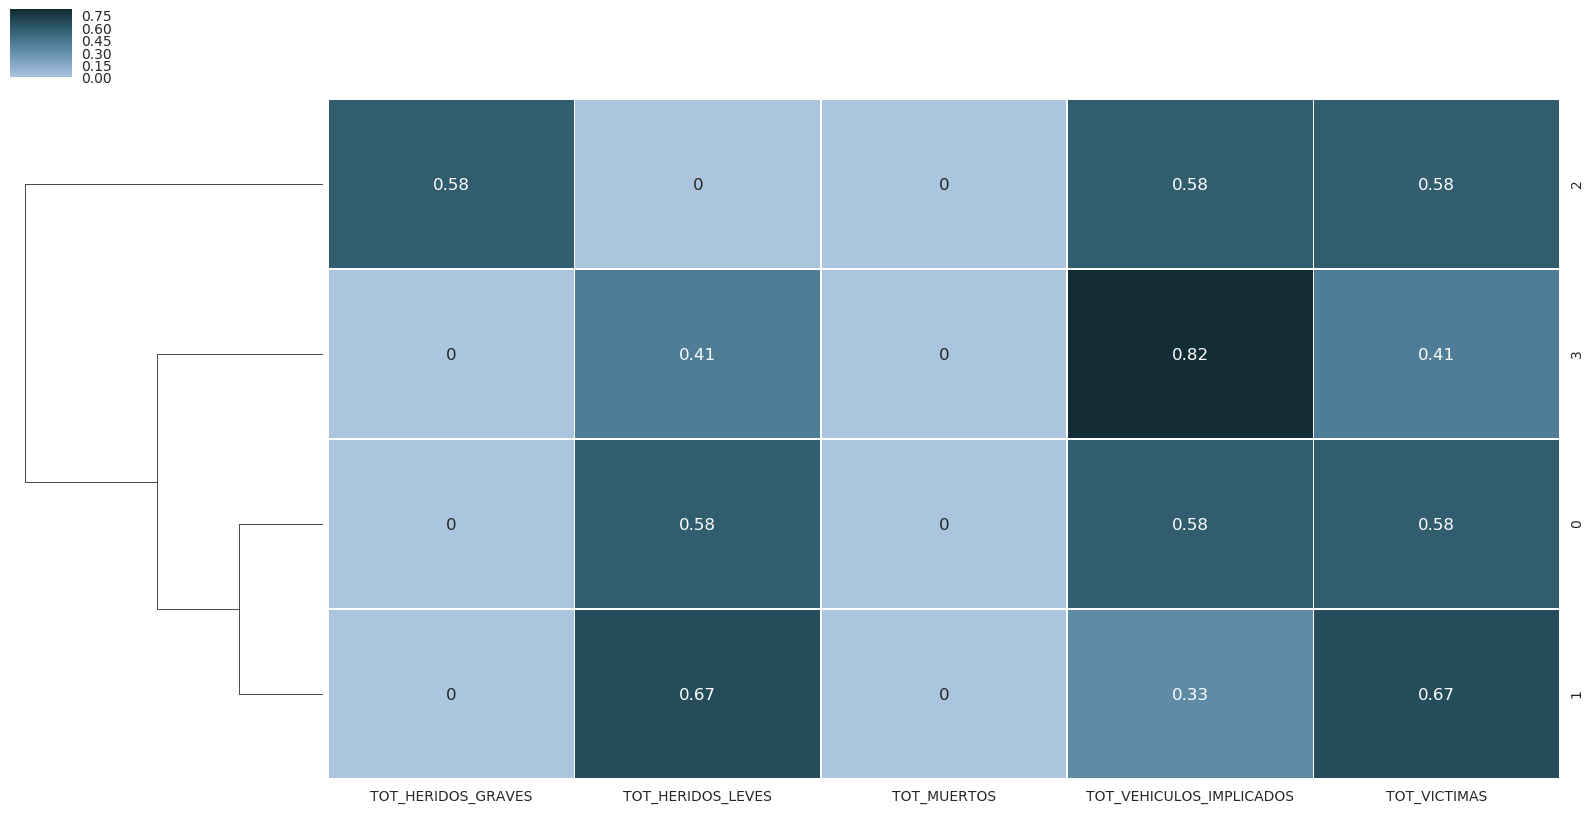
\includegraphics[scale=0.4]{dendrograms/Ward-WetOverturnedAccidents-Dendrogram.png}
		\caption{Dendrograma del algoritmo Ward junto a su heatmap para el tercer caso de estudio.}
	\end{figure}

	\subsection{Interpretación de la segmentación}
	En el apartado final del algoritmo se expondrán las distinciones que se puedan hacer entre los distintos clusters de ambos algoritmos, acompañadas de una explicación apoyada en las gráficas y tablas presentadas anteriormente.
	
	\subsubsection{DBSCAN}
	
	Para el algoritmo DBSCAN nos fijaremos mucho en el heatmap, ya que nos puede aportar una distinción entre los clusters con un solo vistazo. Lo primero a destacar es que en el pequeño subconjunto que supone este caso de estudio no hay ninguna víctima mortal, por lo que todos los valores de la columna de muertes está a 0. Es algo de esperar puesto que no es tan habitual que la gente sufra lesiones tan graves al volcar el coche. Aparte de ello vemos que algunos valores también se repiten para varias variables en el mismo cluster, como el número de víctimas, de vehículos implicados y de heridos graves en el cluster 2. Esto es muy comprensible de nuevo por la dimensión del subconjunto, ya que será difícil encontrar valores muy fluctuantes, sobre todo cuando estamos tratando como en este caso con valores enteros positivos.\\
	
	Realmente lo que se puede decir de un algoritmo no jerárquico en un caso de estudio tan breve es muy limitado. De lo que encontramos en el heatmap también puede parecer curioso el cluster 1, donde hay dos vehículos implicados y una víctima herida leve de media. Como no parece un caso muy normal, es más que probable que haya una cantidad de ejemplos como este muy pequeña, que esté bordando el límite del filtrado realizado.\\
	
	A juzgar por tanto por los valores de las medias, además de utilizando la razón, se puede entender que en la mayoría de los casos cuando se produce un accidente por vuelco es solo un vehículo el que se ve implicado, el que vuelca, y suele ser una persona la que se hiere levemente, la que conduce el vehículo. Esto se corresponde con el cluster 0, y si los valores medios no son exactamente 1 quiere decir que DBSCAN ha decidido agrupar junto a esta presumible mayoría de ejemplos algún otro con dos o más vehículos implicados y el mismo número de heridos leves. De nuevo, con un algoritmo no jerárquico es difícil obtener un análisis elaborado sobre un subconjunto tan escueto.
	
	\subsubsection{Ward}
	
	En primer lugar veamos qué tipo de accidentes son los que están representados en los cuatro clusters que contienen al menos 3 ejemplos del subconjunto. De acuerdo al heatmap, se puede observar que en el cluster 2 se incluyen los accidentes con heridos graves, y que en los cluster 0, 1 y 3 se encuentran accidentes con heridos leves, cuyo número varía inversamente proporcional al número de vehículos implicados para cada cluster, es decir, el que tiene más vehículos provoca menos víctimas y viceversa.\\
	
	Ahora que se ha visto esto sí podremos realizar al menos una aproximación a lo que podría darse en este algoritmo si reducimos el número de clusters como parámetro. Según el dendrograma, la primera asignación que se haría sería reunir los clusters 0 y 1, que son  los más parecidos entre sí puesto que el cluster 3 ya tiene un número de vehículos implicados por encima del resto. No obstante, esta sería la siguiente agrupación según el dendrograma, con el cluster 3. De esta forma estarían reunidos todos aquellos accidentes con heridos leves, y solo quedaría separado el cluster 2 que es el que no tiene heridos leves pero sí tiene graves. Unir ambas agrupaciones finalmente resultaría en una total pérdida de información por parte del algoritmo así que no tiene sentido plantearlo.\\
	
	\subsection{Otras configuraciones de parámetros}
	De nuevo en este apartado no se ofrecerá una configuración distinta para el algoritmo Ward, que ya de por sí es distinta a la del resto de ejecuciones de Ward para otros casos de estudio porque utiliza menos clusters.\\
	
	Con respecto al algoritmo DBSCAN, se ha intentado probar distintas configuraciones de parámetros pero tampoco ha sido posible a causa de errores en tiempo de ejecución, al parecer a causa de modificar el parámetro ``eps'' y aumentarlo por encima de 0.1.
	
\end{document}